\textbf{The objective of the experiment} is to show the behavior of a simple passive
RLC circuit, with a sinusoid of different frequencies as an input signal.
We measure the properties of these circuits, and we analyze the
result of the measurements and how they are represented.


\textbf{A filter} is a network used to select a frequency or range of frequencies while rejecting all others. Usually, they are constructed using active components like transistors or operational amplifiers, however we can also see similar behavior in passive networks of resistors,
capacitors, and inductors. There are four general types. High Pass, Low Pass, Band Pass, and Notch Filters.


In our experiment, we analyze Lo-Pass and Band-Pass filters which are simple in nature, only using passive components such as inductors, capacitors, and resistors.


Furthermore, we will use the Bode plot to analyze the frequency response of these filters, and we will use the Nyquist plot to describe the parametric plot of the frequency response of the filters.

\section{Lo-Pass}
\begin{figure}[H]
    \centering
    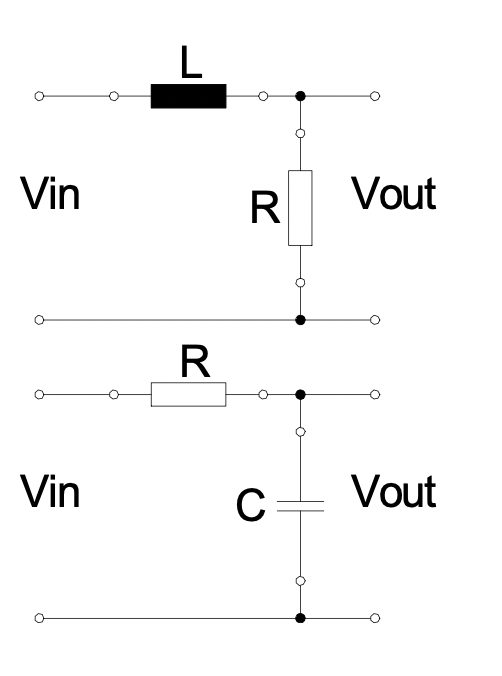
\includegraphics{images/figure_low_pass.png}
    \caption{Low Pass Filter}
\end{figure}


A low pass filter allows low frequencies to pass, while it hinders higher frequencies. With high frequencies, the phase shift of the output signal becomes negative relative to the input signal.


It can be designed using a resistor and a capacitor, or an inductor and a resistor.
In general, we can get the amplitude ratio of the output signal to the input signal by using the following equation:


For an RC circuit, which is what we design in the experiment:
\begin{equation}
    \underline{A} = \frac{V_{out}}{V_{in}} = \frac{1}{1 + j \omega RC}
\end{equation}


To obtain the cutoff frequency, we can use the following equation:
\begin{equation} \label{eq:1.2}
    \underline{f_c} = \frac{1}{2 \pi RC}
\end{equation}


To obtain the amplitude and phase of the output signal, we use the following equations:

\begin{equation}
    |\underline{A}| = \frac{1}{\sqrt{1 + (\omega RC)^2}} \text{ and } \phi = -\arctan(\omega RC)
\end{equation}

\section{Band-Pass}
\begin{figure}[H]
    \centering
    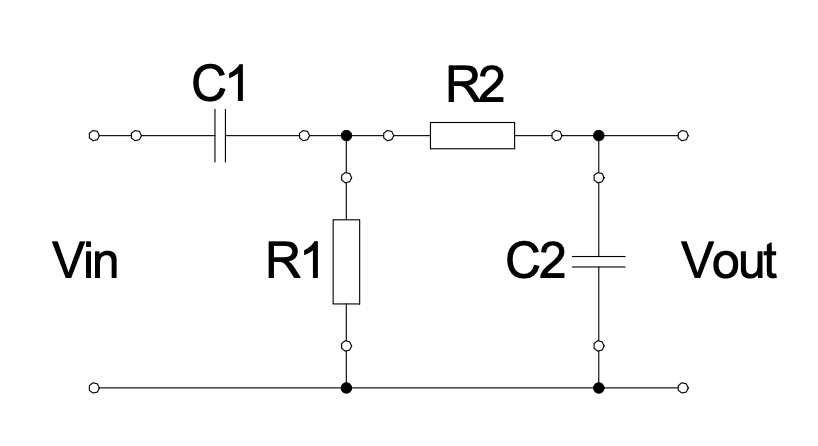
\includegraphics[scale=0.75]{images/figure_band_pass.png}
    \caption{Band Pass Filter}
\end{figure}


A simple band pass filter is simply a combination of a high and low pass filter. It passes through frequencies within a certain range, and attenuates frequencies outside of it.
The formula for the amplitude ratio is the same as the low pass filter, but we have to take into account the high pass filter as well. The formula for the cutoff frequency is also the same as the low pass, and high pass filter (\ref{eq:1.2}).


\section{Obtaining the characteristic output of a filter}


To describe the frequency response of these kinds of networks, we use the Bode plot. We plot the amplitude to frequencies over several decades, and the ratio is calculated.
The unit of the result is \textbf{decibels}, or \textbf{dB}. \textbf{dB} is a logarithmic value used for such purposes. It is defined as:
\begin{equation}
    A = 20 \cdot \log_{10}\frac{V_{out}}{V_{in}}
\end{equation}

\begin{figure}[H]
    \centering
    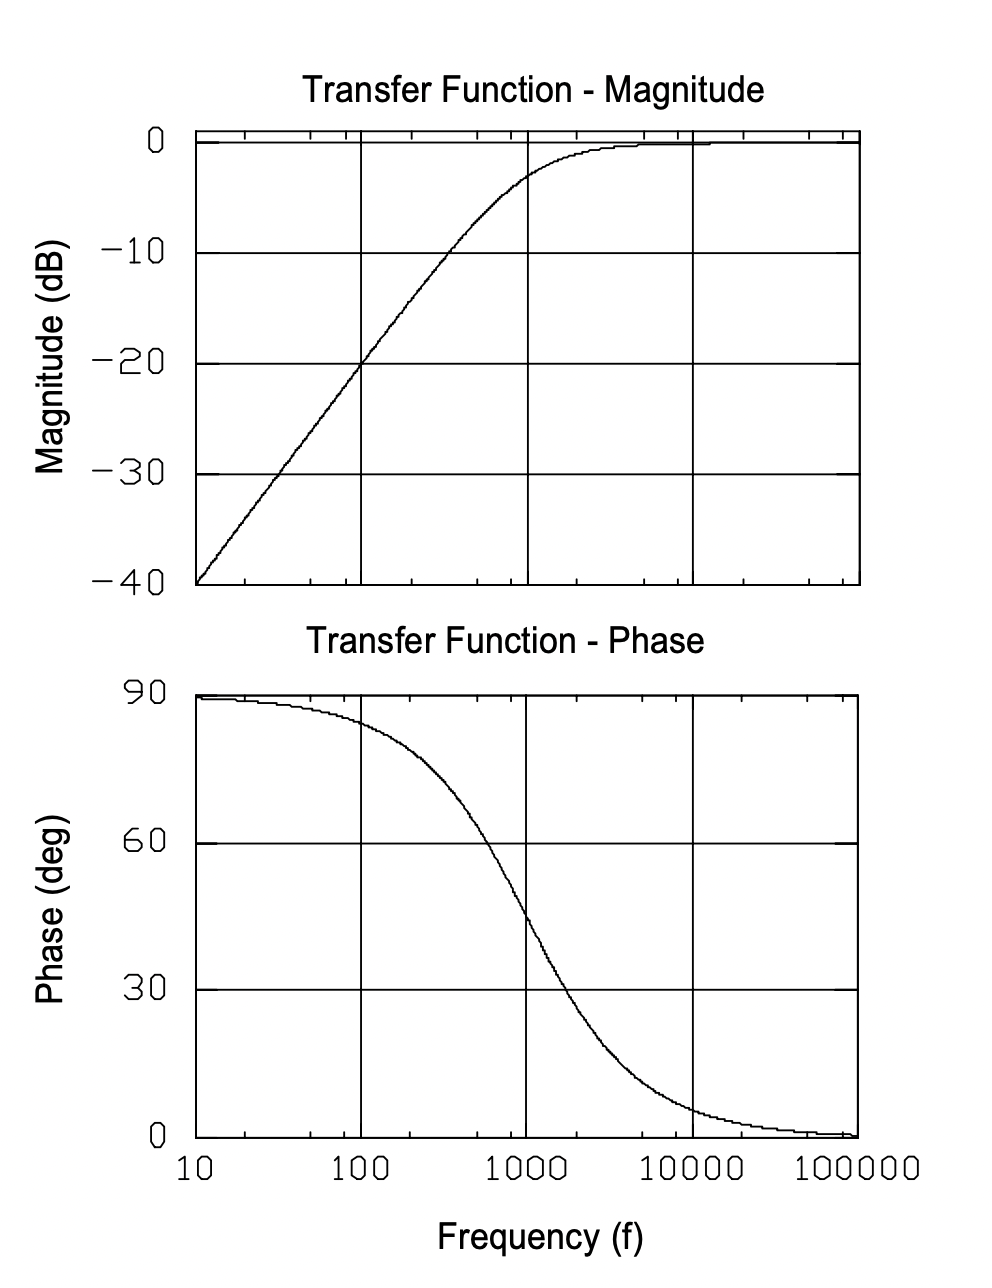
\includegraphics[scale=0.5]{images/bode_plots.png}
    \caption{A bode plot, showing the magnitude plotted against the frequency, and the phase shift plotted against the frequency.}
\end{figure}

The other quantity measured is the phase shift $\phi$ between the input and output signal, taken relative to the input signal. When the output signal is ahead the input, the phase shift $\phi$ is positive, otherwise it is negative.


A \textbf{Nyquist plot} is a parametric plot of a frequency response. In Cartesian coordinates, the real part of the transfer function is plotted on the X axis. The imaginary part is
plotted on the Y axis. The frequency is swept as a parameter, resulting in a plot per frequency.

\begin{figure}[H]
    \centering
    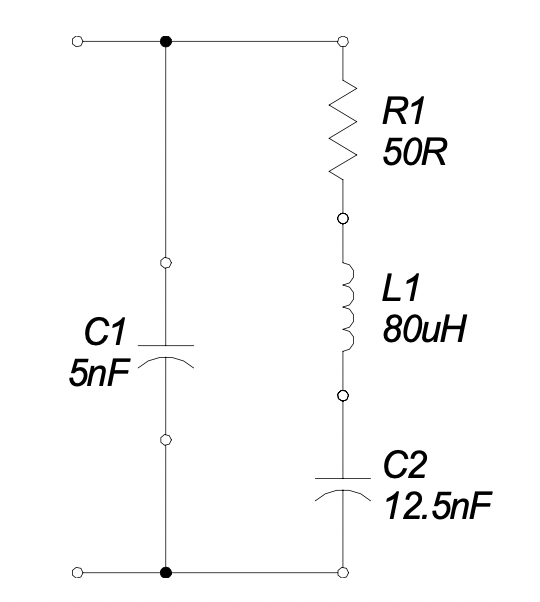
\includegraphics[scale=0.5]{images/nyquist_rlc_circuit.png}
    \caption{An RLC circuit with a capacitor in parallel.}
\end{figure}

We wish to find how the complex conductance changes when $\omega$ changes, given that the impedance for the RLC series circuit is
\[\underline{Z_S} = R_1 + j(\omega L_1 - \frac{1}{\omega C_2})\] and with the parallel capacitor the admittance is \[\underline{Y_{all}} = j\omega C_1 + \frac{1}{\underline{Z_S}}\]

When varying $\omega$, a Nyquist plot is generated. The right plot is \(\frac{1}{Y_{all}}\)

\begin{figure}[H]
    \centering
    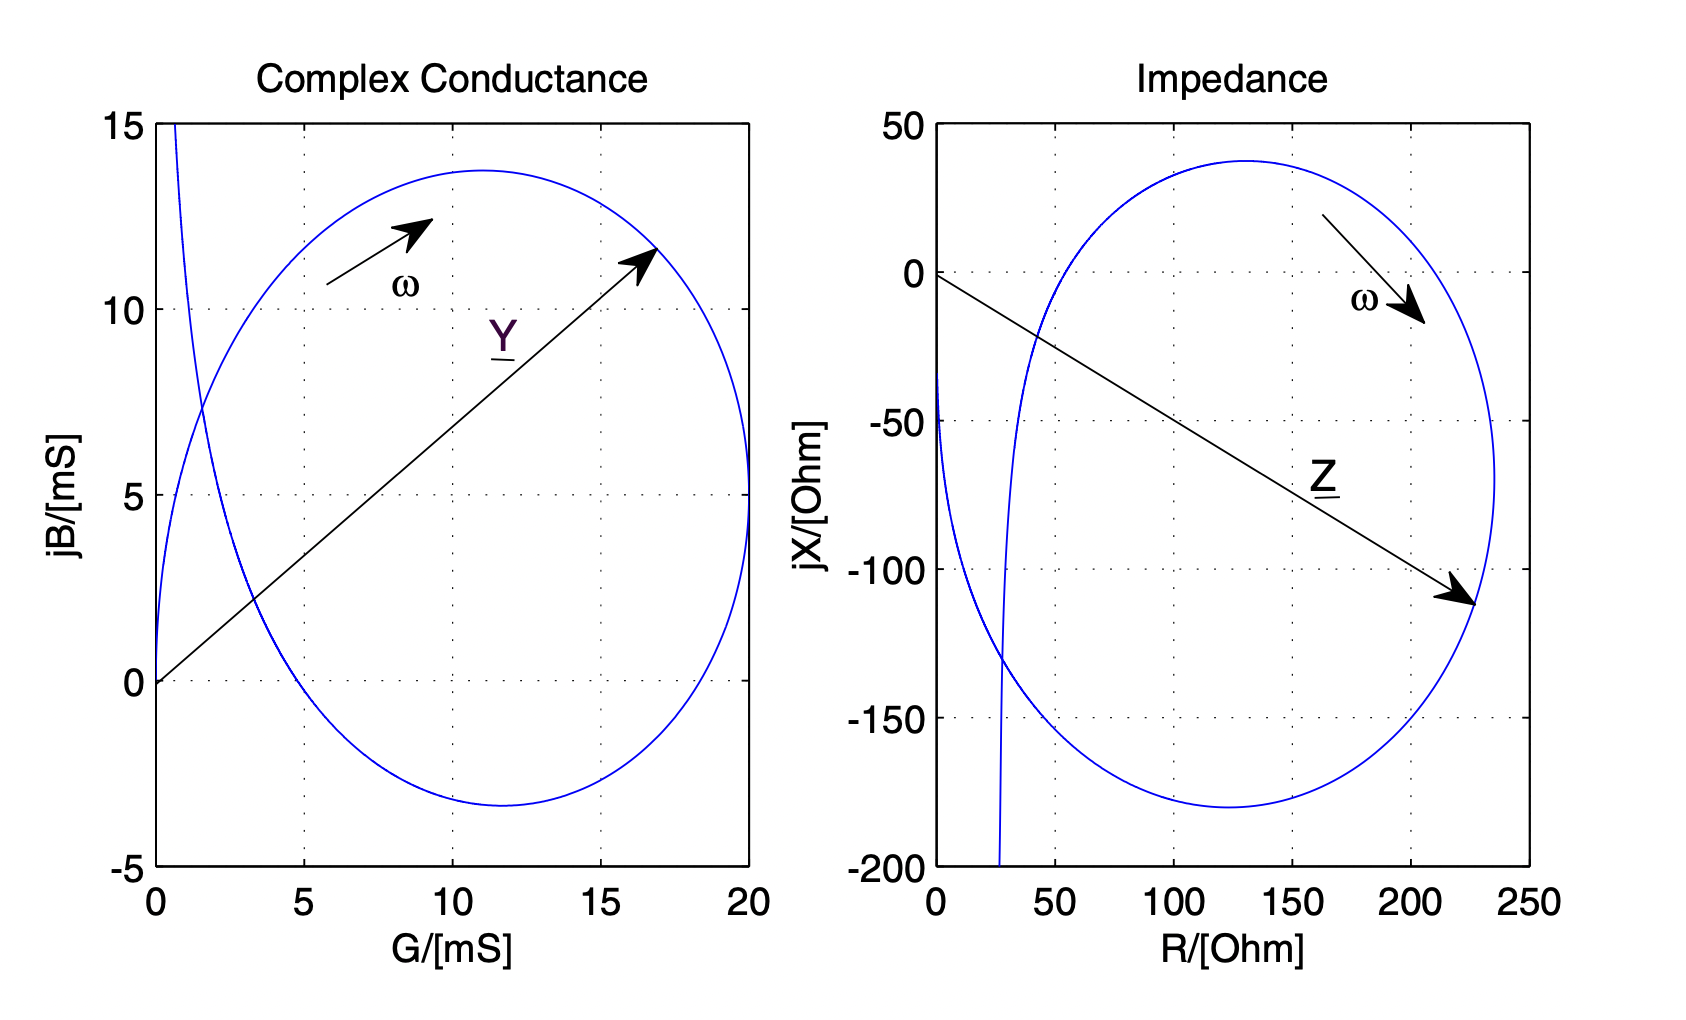
\includegraphics[scale=0.35]{images/nyquist_plot_rlc.png}
    \caption{The nyquist plot of the RLC circuit.}
\end{figure}
